\documentclass[11pt]{article}
\usepackage[a4paper,margin=25mm]{geometry}
\usepackage{amsmath,amssymb,amsthm,booktabs,array,enumitem,hyperref,tikz,microtype,needspace,placeins}
\usetikzlibrary{arrows.meta,positioning}
\renewcommand{\topfraction}{0.85}
\renewcommand{\textfraction}{0.10}
\hypersetup{pdftitle={Pure Nash Equilibrium Existence in Edge-Ranking Flow Allocation Games is Sigma2p-Complete},pdfauthor={Zhiyan Lin},pdfsubject={Preprint v0.1: pure Nash equilibrium existence},colorlinks=true,linkcolor=blue!45!black,citecolor=blue!45!black,urlcolor=blue!45!black}
\newtheorem{theorem}{Theorem}
\newtheorem{lemma}[theorem]{Lemma}
\newtheorem{proposition}[theorem]{Proposition}
\newtheorem{corollary}[theorem]{Corollary}
\newcommand{\sig}{\Sigma^{\mathrm p}_2}
\newcommand{\pne}{\mathrm{PNE}}
\newcommand{\pos}[1]{(#1)_+}
\title{Pure Nash Equilibrium Existence in Edge-Ranking\ Flow Allocation Games is $\sig$-Complete}
\author{Zhiyan Lin}
\date{12 October 2026\\\small Preprint v0.1 -- release candidate}
\begin{document}
\maketitle
\begin{abstract}
We give a polynomial-time reduction proving that pure Nash equilibrium existence in edge-ranking flow allocation games is $\sig$-complete, with every vertex strategic and with greatest-fixed-point clearing. The main ingredient is a two-edge strategic threshold gate: a private lossy return cycle makes one order strictly dominant, while the external output is exactly $\pos{t-H}$ for external inflow $t$ and threshold $H$. The dominance proof allows arbitrary feedback from the surrounding network. Substituting these gates into a previously proposed guarded quantified-Boolean reduction removes its fixed-priority assumption. The reduction uses a simple directed graph, integral capacities and supplies bounded polynomially in the formula size, and no prescribed strategies.
\end{abstract}

\section{Introduction}
A financial network may contain cyclic obligations: a payment received by one institution can fund further payments and eventually return through the network. In a flow allocation game, vertices strategically choose how to distribute available flow. Under an edge-ranking strategy, a vertex orders its outgoing edges and fills them sequentially up to their capacities. Its utility is its total outgoing flow. A clearing rule is needed because cyclic obligations may admit several consistent flows; the model studied here selects the coordinatewise greatest feasible fixed point.

Bertschinger, Hoefer, and Schmand~\cite{bhs} introduced and analyzed this model. Their results distinguish flexible rankings of individual units of flow from rankings of whole edges. Unit-ranking games always admit a strong equilibrium maximizing total flow. Edge-ranking games can lack even a pure Nash equilibrium. For the latter games, the authors established strong NP-hardness of equilibrium existence and observed membership in $\sig$, leaving the exact classification open in Remark~3 of the journal-format manuscript (Remark~21 of arXiv v3). Polynomial-time clearing for a fixed edge-ranking profile does not make equilibrium verification easy: a vertex may have factorially many rankings.

Earlier, Guha, Kupferman, and Vardi~\cite{gkv} proved $\sig$-completeness of equilibrium existence in multi-player flow games. Their acyclic networks allow a player to control several vertices and optimize flow at a designated target, using general allocation policies. That classification does not apply directly to the present one-vertex-per-player permutation game. Indeed, in the present model every profile on an acyclic graph is a strong equilibrium~\cite[Proposition~1]{bhs}. Thus a matching complexity class in the earlier model is not a prior solution of this question.

Our main result is the following classification: \emph{pure Nash equilibrium existence in edge-ranking flow allocation games is $\sig$-complete, even on simple directed graphs with polynomially bounded integral parameters and with every vertex strategic}. Theorem~\ref{thm:main} gives the precise statement and proof. This resolves the decision problem listed as problem~107 in the public MOR open-problem collection.

The contribution builds on three sources. Bertschinger, Hoefer, and Schmand~\cite{bhs} provide the model, polynomial-time greatest clearing, and the no-equilibrium alarm. The public partial-progress note~\cite{progress} provides a guarded quantified-Boolean reduction with prescribed priorities at auxiliary vertices, together with the alarm's corrected zero-input behavior. Kanellopoulos, Kyropoulou, and Zhou~\cite[Section~6]{kkz} already use lossy private return pairs to implement subtraction thresholds with priority incentives, in a different priority-proportional model. We establish a uniform strict-dominance bound that remains valid when a deviation changes the surrounding feedback, and use it to complete the guarded reduction with every vertex strategic. The new ingredient is the joint guarantee of threshold output and strategic incentives under feedback, rather than the subtraction formula alone. A signal lemma valid for every tester and fanout permutation then establishes correctness of the completed reduction.

More specifically, the private circulation in Lemma~\ref{lem:gate} gives the desired order utility at least $M$, whereas any other order gives utility at most a uniform inflow bound $T<M$. The gate uses no external subsidy and has zero logical output at zero external input. This avoids the false activation identified in the earlier proposed priority lock in~\cite{progress}. The guarantee uses greatest clearing and outgoing-flow utility. In contrast, the strategies in~\cite{kkz} allow ties, utilities are total assets, and clearing is required to be proper; its equilibrium-existence hardness theorem does not classify the present model.

The resulting classification answers the original decision question, rather than a bounded-dimensional instance or a fixed-priority variant. It implies that an NP classification would collapse the polynomial hierarchy to its first level; it does not establish an unconditional separation from NP. The construction remains polynomial in size even when its integer parameters are written in unary.

Section~2 fixes the model and complexity source problem. Section~3 proves the strategic threshold lemma. Section~4 records the conditional alarm with complete finite checks. Section~5 constructs the reduction, and Section~6 proves its correctness. Section~7 concludes. Supplementary computational checks appear in Appendix~\ref{app:checks}; the accompanying repository records reproduction instructions and source provenance.

\section{Preliminaries}
Let $G=(V,E)$ be a finite directed graph, $c_e$ a positive integer capacity for each edge $e$, and $b_v$ a nonnegative integer supply for each vertex $v$. Write $\pos{x}=\max\{x,0\}$ for the positive part of a real number $x$. Write $E^+(v)$ and $E^-(v)$ for the outgoing and incoming edge sets. Zero-capacity edges in an original input can be deleted: they always carry zero flow and consume no supply, so deleting them from every ranking preserves clearing and all utilities, and rankings on the reduced graph can be lifted by inserting them anywhere. Thus the positive-capacity convention loses no instances. Every vertex is a player; a sink has the unique empty strategy. A strategy $\pi_v$ is a permutation of $E^+(v)$, and $\pi=(\pi_v)_{v\in V}$ is a profile.

For a vector $f\in\prod_{e\in E}[0,c_e]$, the available inflow at $v$ is
\[
 a_v(f)=b_v+\sum_{e\in E^-(v)} f_e.
\]
If $\pi_v=(e_1,\ldots,e_k)$, where $k=|E^+(v)|$, the allocation map is explicitly
\begin{equation}\label{eq:clearing}
 (F_\pi(f))_{e_j}
 =\min\!\left\{c_{e_j},\,
 \left(b_v+\sum_{e\in E^-(v)}f_e-\sum_{h<j}c_{e_h}\right)_+\right\},
 \qquad 1\le j\le k.
\end{equation}
Thus each vertex fills its edges in order, retaining excess only after every outgoing edge is saturated. A feasible clearing flow is a fixed point $f=F_\pi(f)$. The monotonicity of greedy allocation gives a greatest fixed point $\widehat f(\pi)$; equivalently, the fixed points form a complete lattice~\cite[Theorem~1]{bhs}. Utilities and equilibrium are defined by
\begin{equation}\label{eq:pne}
 u_v(\pi)=\sum_{e\in E^+(v)}\widehat f_e(\pi),\qquad
 \pi\text{ is a }\pne\ \Longleftrightarrow\
 u_v(\pi)\ge u_v(\pi'_v,\pi_{-v})\quad\text{for all }v,\pi'_v.
\end{equation}
Here $\pi_{-v}$ denotes the strategies of all other vertices. In particular, utility is outgoing flow, not retained equity. A strictly dominant order yields strictly larger utility than every alternative against every fixed profile of the other players, with the clearing state recomputed after a deviation.

The decision problem $\mathrm{ER\text{-}NE}$ asks whether an input game has a pure Nash equilibrium. The following upper bound is already observed in~\cite[Remark~3]{bhs}; we include its short justification.
\begin{proposition}\label{prop:upper}
$\mathrm{ER\text{-}NE}$ belongs to $\sig$.
\end{proposition}
\begin{proof}
A profile, a player, and one alternative permutation all have polynomial-length descriptions. The TopCycleIncrease algorithm computes greatest clearing in strongly polynomial time for any fixed edge-ranking profile~\cite[Proposition~5]{bhs}. Consequently the inequality in~\eqref{eq:pne} is a polynomial-time predicate. Existentially quantify the profile and universally quantify a player and an alternative permutation. The predicate first rejects invalid existential profile encodings; for a valid profile, it is true on invalid universal encodings and otherwise evaluates the deviation inequality. This is a $\sig$ decision procedure.
\end{proof}

Our source problem is the truth of
\begin{equation}\label{eq:qbf}
 \exists X\ \forall Y\ \neg F(X,Y),
\end{equation}
where $X=(x_1,\ldots,x_n)$, $Y=(y_1,\ldots,y_r)$, and $F$ is a CNF formula with $m$ clauses, each containing at most three literals. We may assume $r,m\ge1$. Repeated literals within a clause are removed; a tautological clause is allowed. The problem is $\sig$-complete. For clarity, one can obtain this formulation from the polynomial-predicate characterization of the hierarchy~\cite{stockmeyer}: given $\exists X\forall Y\,P(X,Y)$, encode the circuit computing $\neg P$ by a Tseitin 3-CNF $F(X,Y,Z)$ with
\[
 \neg P(X,Y)\ \Longleftrightarrow\ \exists Z\,F(X,Y,Z).
\]
Then $\forall Y\,P(X,Y)$ is equivalent to $\forall(Y,Z)\,\neg F(X,Y,Z)$. The auxiliary circuit variables join the universal block. A dummy universal variable and a tautological clause give the stated nonemptiness assumptions. Thus there is no unjustified conversion of a universally quantified CNF into an equivalent 3-CNF.

\section{A strictly dominant threshold gate}
The next lemma gives the uniform strict-dominance guarantee needed here for the lossy-return mechanism related to~\cite{kkz}, using ordinary strategic vertices. Its inflow bound is required for all feasible flows, not merely at one intended profile. Such a bound is always available from the external incoming capacities.

\Needspace{19\baselineskip}
\begin{lemma}\label{lem:gate}
Let $v$ have exactly two outgoing edges: $v\to w$ of capacity $M+H$ and $v\to z$ of capacity $C$. The private vertex $w$ has supply zero and no incident edges except $v\to w$ and $w\to v$, the latter of capacity $M$. Let $t$ denote the supply of $v$ plus all its incoming flow other than $w\to v$. Suppose $0\le t\le T$ in every feasible flow under every strategy profile, and choose $H\ge0$, $M>T$, and $C>T$.

Ranking $v\to w$ first is strictly dominant. In greatest clearing under this order, the return flow is $M$, the output to $z$ is $\pos{t-H}$, and $u_v=M+t$. If $v\to z$ is ranked first, every feasible fixed point has return flow zero and $u_v=t\le T$.
\end{lemma}
\begin{proof}
Write $q=f_{wv}$, $\ell=f_{vw}$, and $s=f_{vz}$. The private vertex enforces $q=\min\{\ell,M\}$.

First rank $v\to w$ first and consider the greatest fixed point. If $q<M$, then $\ell=q<M\le M+H$. The first edge is unsaturated, so $\ell=t+q$, implying $t=0$ and $s=0$. Replace both private edge flows by $M$ and leave every other edge unchanged. At $v$, inflow is now $M$, all of which goes to $w$; at $w$, all $M$ units return. The output $s$ remains zero. Thus the modified vector is a feasible fixed point strictly larger on two coordinates, contradicting greatestness. Therefore $q=M$. Greedy allocation now gives
\[
 \ell=M+\min\{t,H\},\qquad s=\pos{t-H},\qquad u_v=M+t,
\]
because $s\le T<C$ and total outgoing capacity exceeds $M+t$.

Next rank $v\to z$ first and consider any fixed point. Suppose $q>0$. Then $\ell>0$, so the first edge must be saturated: $s=C$. Since $t+q\le T+M<C+M\le C+M+H$, the total outgoing capacity is not exhausted, and flow conservation at $v$ gives $t+q=C+\ell$. As $q\le\ell$, this implies $t\ge C$, contradicting $t\le T<C$. Hence $q=0$. Now $t<C$, so $s=t$, $\ell=0$, and $u_v=t\le T$.

The external inflow may change when $v$ switches order. This causes no difficulty: the first order always yields at least $M$, while the second always yields at most $T<M$. Strict dominance follows against every surrounding profile.
\end{proof}

\begin{figure}[ht]
\centering
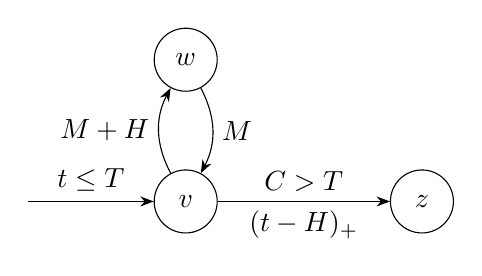
\begin{tikzpicture}[>=Stealth,vertex/.style={draw,circle,minimum size=8mm}]
\node[vertex] (v) at (0,0) {$v$};
\node[vertex] (w) at (0,1.8) {$w$};
\node[vertex] (z) at (3,0) {$z$};
\draw[->] (-2,0)--node[above] {$t\le T$}(v);
\draw[->] (v) to[bend left=28] node[left] {$M+H$}(w);
\draw[->] (w) to[bend left=28] node[right] {$M$}(v);
\draw[->] (v)--node[above] {$C>T$} node[below] {$\pos{t-H}$}(z);
\end{tikzpicture}
\caption{A strategic threshold gate. Edge labels above edges are capacities; the output label below the horizontal edge is its clearing flow when the private edge has priority. The return cycle contains no fixed supply.}
\label{fig:gate}
\end{figure}

The private vertex retains $\min\{t,H\}$ after its return edge saturates. The gate therefore uses a controlled loss of logical flow, not a general compiler preserving an arbitrary prescribed ordering. Its private circulation raises the owner's utility without creating external output at zero input. The proof specifically uses greatest clearing: it does not claim the same behavior for least clearing.

The uniform margin is relevant when feedback changes the input. To see this directly, take zero supplies, a third vertex $z$ with the sole edge $z\to v$ of capacity $T>0$, and gate parameters $H>0$, $C>T$, with any $M>0$. If the private edge is first, greatest clearing gives $q=M$ and $t=\min\{(t-H)_+,T\}$, hence $t=0$ and $u_v=M$. The derivation of this output formula used $C>T$ but not $M>T$. If the external edge is first, $q=0$ and greatest clearing sends $T$ around $v\to z\to v$, so $u_v=T$. Consequently $M<T$ can make the desired order worse and $M=T$ can make it only tied. The condition $M>T$ excludes both failures. This example explains the strengthened guarantee; it is not needed for the hardness reduction.

\section{A conditional no-equilibrium module}
We use the alarm in~\cite[Proposition~9]{bhs}, with its zero-input behavior as recorded in~\cite{progress}. It has vertices $a_1,\ldots,a_7$ and the edges in Table~\ref{tab:alarmedges}. Only $a_1,a_2,a_3$ have two outgoing edges. All supplies inside the module are zero; external input may enter $a_2$ and $a_3$.

When this module is embedded in a larger network, fix its incoming edge flows. Because no edge leaves the module, the restriction of the global greatest clearing flow is the module's greatest fixed point for those inputs. Otherwise, replace its internal flow by the strictly larger greatest fixed point, leaving every external edge unchanged. The result is a global fixed point larger than the global greatest one, a contradiction. Thus the following local payoff calculation remains valid inside the reduction.

\begin{table}[ht]
\centering
\begin{tabular}{cc@{\qquad}cc}
\toprule Edge&Capacity&Edge&Capacity\\\midrule
$a_5\to a_2$&1&$a_2\to a_5$&6\\
$a_2\to a_1$&6&$a_4\to a_2$&2\\
$a_1\to a_4$&4&$a_1\to a_6$&4\\
$a_6\to a_3$&2&$a_3\to a_1$&6\\
$a_7\to a_3$&1&$a_3\to a_7$&6\\\bottomrule
\end{tabular}
\caption{Edges of the conditional alarm. No edge leaves the module.}\label{tab:alarmedges}
\end{table}

\Needspace{7\baselineskip}
\begin{lemma}\label{lem:alarm}
With zero external input, the alarm has a pure Nash equilibrium. With external input two at each of $a_2,a_3$, it has no pure Nash equilibrium.
\end{lemma}
\begin{proof}
At zero input, take the priorities $a_1\to a_4$ first, $a_2\to a_1$ first, and $a_3\to a_7$ first. Greatest clearing sends two units around $a_1\to a_4\to a_2\to a_1$ and one around $a_3\to a_7\to a_3$. To verify greatestness directly, the return capacities bound these cycles by two and one; the priority edges then prevent any other cycle from carrying flow. Utilities of the three strategic vertices are $(2,2,1)$. Their respective unilateral reversals yield own utilities $0,1,0$, so none improves.

For external inputs $(2,2)$, Table~\ref{tab:payoffs} lists the utilities of $(a_2,a_3)$ for all eight profiles. These values follow by substituting the greedy equations along the degree-one return paths. For example, if $a_1\to a_4$, $a_2\to a_1$, and $a_3\to a_1$ are all first, the eight units reaching $a_1$ send four along each of its outgoing edges; two return to each of $a_2,a_3$, and both attain utility four. When $a_2$ instead prioritizes $a_5$, one unit returns along that private pair and the greedy equations give utilities $(5,2)$. The other entries follow from the same two choices and the symmetry exchanging the left and right halves. In either table every cell has a strictly profitable row or column switch. Hence no profile is a pure Nash equilibrium, regardless of $a_1$'s order.
\end{proof}

\begin{table}[ht]
\centering
\begin{tabular}{ccccc}
\toprule
&\multicolumn{2}{c}{$a_1\to a_4$ first}&\multicolumn{2}{c}{$a_1\to a_6$ first}\\
$a_2$ first target&$a_3\to a_1$&$a_3\to a_7$&$a_3\to a_1$&$a_3\to a_7$\\\midrule
$a_1$&$(4,4)$&$(4,3)$&$(4,4)$&$(2,5)$\\
$a_5$&$(5,2)$&$(3,3)$&$(3,4)$&$(3,3)$\\\bottomrule
\end{tabular}
\caption{Alarm utilities $(u_{a_2},u_{a_3})$ under inputs $(2,2)$. Each column specifies the first target of $a_3$.}\label{tab:payoffs}
\end{table}

\section{Construction of the all-strategic game}
Fix a source formula~\eqref{eq:qbf}. A value track is indexed by a variable and a value $b\in\{0,1\}$. A track targets clause $C_j$ precisely when setting its variable to $b$ makes a literal of $C_j$ true. Each such target is included once, even if the clause repeats that literal. Define
\[
 R=5,\qquad K=m+r,\qquad B=R(m+1)+1,\qquad S=rB.
\]
Here $R$ is the logical block size, $K$ is the number of collectors, $B$ is a track input block, and $S$ is the tester supply. These parameters separate full logical blocks from feedback residue. The block size $R=5$ splits into two units for each alarm input and one unit returned to the tester. Every track has at most $m+1$ targets, so $B=R(m+1)+1$ leaves a threshold of at least one at every track gate. A full input of $B$ survives that threshold with exactly enough flow to fill all target edges; any residual input of at most one is eliminated. The tester has supply $rB$, so exactly its first $r$ edges receive full blocks. Variable guards force those $r$ edges to represent a consistent assignment. Figure~\ref{fig:reduction} summarizes the construction; private cycles inside threshold gates are omitted.

\begin{figure}[htbp]
\centering
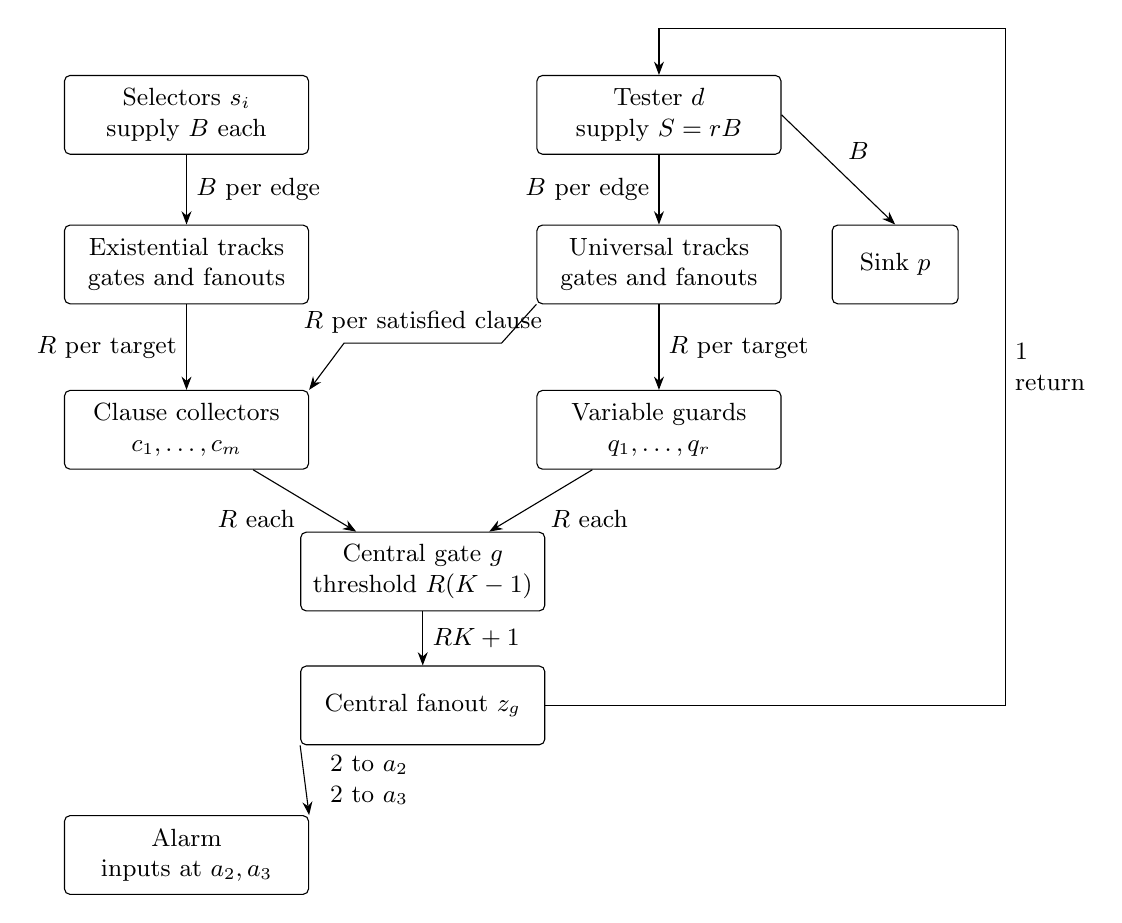
\begin{tikzpicture}[>=Stealth,block/.style={draw,rounded corners=2pt,align=center,minimum width=31mm,minimum height=10mm,font=\small},every edge/.style={draw,->},font=\small]
\node[block] (sel) at (0,0) {Selectors $s_i$\\supply $B$ each};
\node[block] (test) at (6,0) {Tester $d$\\supply $S=rB$};
\node[block] (xt) at (0,-1.9) {Existential tracks\\gates and fanouts};
\node[block] (yt) at (6,-1.9) {Universal tracks\\gates and fanouts};
\node[block,minimum width=16mm] (sink) at (9,-1.9) {Sink $p$};
\node[block] (cl) at (0,-4) {Clause collectors\\$c_1,\ldots,c_m$};
\node[block] (gu) at (6,-4) {Variable guards\\$q_1,\ldots,q_r$};
\node[block] (gate) at (3,-5.8) {Central gate $g$\\threshold $R(K-1)$};
\node[block] (fan) at (3,-7.5) {Central fanout $z_g$};
\node[block] (alarm) at (0,-9.4) {Alarm\\inputs at $a_2,a_3$};
\draw[->] (sel)--node[right] {$B$ per edge}(xt);
\draw[->] (test)--node[left] {$B$ per edge}(yt);
\draw[->] (test.east)--node[above right] {$B$}(sink.north);
\draw[->] (xt)--node[left] {$R$ per target}(cl);
\draw[->] (yt)--node[right] {$R$ per target}(gu);
\draw[->] (yt.south west)--(4,-2.9)--node[above] {$R$ per satisfied clause}(2,-2.9)--(cl.north east);
\draw[->] (cl)--node[below left] {$R$ each}(gate);
\draw[->] (gu)--node[below right] {$R$ each}(gate);
\draw[->] (gate)--node[right] {$RK+1$}(fan);
\draw[->] (fan.south west)--node[pos=0.5,right,xshift=2mm,align=left] {$2$ to $a_2$\\$2$ to $a_3$}(alarm.north east);
\draw[->] (fan.east)--(10.4,-7.5)--node[right,align=left] {$1$\\return}(10.4,1.1)--(6,1.1)--(test.north);
\end{tikzpicture}
\caption{The complete reduction at the module level. Labels are edge capacities; arrows between families denote the corresponding sets of edges. Private return pairs are as in Figure~\ref{fig:gate}. Universal tracks also target the clauses they satisfy. The alarm has no outgoing connection to the rest of the network. The capacity-one return edge is the only feedback edge outside the threshold gates and the alarm.}\label{fig:reduction}
\end{figure}

Every unspecified supply is zero. All vertices, including all auxiliary vertices, choose arbitrary permutations of their outgoing edges.

\paragraph{Selectors and tester.}
For each existential variable $x_i$, create a vertex $s_i$ with supply $B$ and outgoing edges of capacity $B$ to its two track vertices $X_{i,0},X_{i,1}$. There are no incoming edges to $s_i$. Create a tester $d$ with supply $S$, outgoing edges of capacity $B$ to the $2r$ universal tracks $Y_{\ell,b}$, and one more edge of capacity $B$ to a new sink $p$. Its only incoming edge will have capacity one.

\paragraph{Track gates and fanouts.}
For every track vertex $v$, let $L_v$ be its target list. For an existential track it consists of its satisfied clauses. For a universal track $Y_{\ell,b}$ it also includes guard $q_\ell$. Let $k_v=|L_v|$, so $0\le k_v\le m+1$, and set
\[
 H_v=B-Rk_v\ge1.
\]
Apply Lemma~\ref{lem:gate} at $v$ with $T=B$, $M=C=B+1$, and threshold $H_v$. Its private return vertex and output vertex $z_v$ are new. From $z_v$ create an edge of capacity $R$ to each target collector in $L_v$. Thus its total outgoing capacity is $Rk_v$. When $k_v=0$, $z_v$ is a sink. Each track has just one external incoming edge, of capacity $B$, so the bound $T=B$ holds under every profile. We refer to the orders putting private edges first as the gate orders.

\paragraph{Collectors and central gate.}
Create one collector $c_j$ per clause and one guard collector $q_\ell$ per universal variable. Every collector has a single outgoing edge of capacity $R$ to a central gate $g$. Consequently the external inflow to $g$ is at most $RK$ under every profile. Apply Lemma~\ref{lem:gate} at $g$ with
\[
 T=RK,\qquad M=C=RK+1,\qquad H_g=R(K-1).
\]
The output vertex $z_g$ has three outgoing edges: capacity two to $a_2$, capacity two to $a_3$, and capacity one to $d$. Their total capacity is $R$. Add the alarm from Section~4, with no further connections.

\paragraph{Size and integrality.}
All vertices introduced for different gates are distinct. There are $2(n+r)$ track gates, $n$ selectors, $K$ collectors, one central gate, the tester, its sink, and seven alarm vertices. Each gate uses three vertices including its input and fanout vertices. Clause-target edges are linear in the literal occurrences; the guard-target edges number $2r$. The construction has polynomially many vertices and edges, has no self-loops or parallel edges, and all capacities are $O(m+r)$. The largest supply is $S=O(r(m+1))$. Writing all numbers in unary therefore still gives a polynomial-size reduction.

\FloatBarrier
\section{Correctness}
Call a profile normalized if every track gate and the central gate uses its gate order. No restriction is imposed on any other vertex's strategy. Lemma~\ref{lem:gate} implies that every pure Nash equilibrium is normalized, regardless of the other players' strategies.

The next lemma handles the return edge to the tester, including all possible fanout deviations. A prefix means the ordered list of the first $r$ outgoing edges of $d$. It is called consistent if it consists of exactly one track for each universal variable and does not contain the edge to $p$.

\begin{lemma}\label{lem:signals}
Fix a normalized profile. Let $\alpha_i$ be the value of the track ranked first by $s_i$, and let $Q$ be the tester prefix. Define $\sigma=1$ if $Q$ is consistent and its represented assignment $\beta$ satisfies $F(\alpha,\beta)$; otherwise define $\sigma=0$. In greatest clearing, the flow from $z_g$ to $d$ is exactly $\sigma$, the inputs to $(a_2,a_3)$ are $(2\sigma,2\sigma)$, and
\begin{equation}\label{eq:tester}
 u_d=S+\sigma.
\end{equation}
For fixed selector and tester orders, all track-fanout and central-fanout flows, and their owners' utilities, are independent of every fanout order and every alarm order.
\end{lemma}
\begin{proof}
Let $\rho$ be the clearing flow on $z_g\to d$. Its capacity gives $0\le\rho\le1<B$. Available flow at $d$ is $rB+\rho$, so the first $r$ outgoing edges are filled to $B$. Only the next edge can receive any further flow, and it receives at most one. There are $2r+1$ outgoing edges; their total capacity exceeds $rB+1$. This proves $u_d=S+\rho$.

An existential selector supplies $B$ to exactly its first track and zero to the other. Every universal track receives either $B$ (when in $Q$) or at most one. By Lemma~\ref{lem:gate}, a track receiving $B$ outputs $B-H_v=Rk_v$, while a track receiving at most one outputs zero because $H_v\ge1$. Thus each track fanout receives either zero or exactly its entire outgoing capacity. Its edges are therefore all zero or all saturated, independently of its permutation.

Each collector consequently receives a sum of whole $R$-blocks. Its outgoing edge is $R$ precisely when at least one of its target tracks is full, and otherwise is zero. If $j$ collectors are active, the external input to $g$ is $Rj$, where $0\le j\le K$. Lemma~\ref{lem:gate} gives its output
\[
 \pos{Rj-R(K-1)}=
 \begin{cases}R,&j=K,\\0,&j<K.\end{cases}
\]
The central fanout receives either zero or its entire outgoing capacity. It sends $(2,2,1)$ to $(a_2,a_3,d)$ if all collectors are active, and $(0,0,0)$ otherwise, under every permutation.

All $r$ guards are active only if $Q$ contains at least one track for each universal variable. Since $Q$ contains exactly $r$ edges, this is equivalent to consistency. Under consistency, a clause collector is active exactly when the existential assignment $\alpha$ and the represented universal assignment $\beta$ satisfy that clause. Thus all $K$ collectors are active exactly when $\sigma=1$. It follows that $\rho=\sigma$, proving~\eqref{eq:tester} and the asserted alarm inputs.

This argument applies to every normalized profile, and it used only the capacity bound on $\rho$, never an assumption that the return is initially zero. For fixed selector and tester orders, the full tracks and then all fanout flows are fixed by the argument. Alarm vertices have no outgoing edges to the rest of the network. Consequently changing any fanout or alarm permutation cannot change these logical flows or the utilities of the fanout owners.
\end{proof}

The last paragraph is important at inactive fanouts: a claim that a vertex currently has zero inflow would alone be insufficient to rule out a deviation that creates a new clearing cycle. Lemma~\ref{lem:signals} establishes invariance after recomputing greatest clearing for every such deviation.

\Needspace{7\baselineskip}
We can now give the complete classification for the original model.
\begin{theorem}\label{thm:main}
Deciding whether an edge-ranking flow allocation game admits a pure Nash equilibrium is $\sig$-complete. Hardness holds for simple directed graphs with nonnegative integral supplies and positive integral capacities that are polynomially bounded in the size of the reduced formula. Every vertex is strategic.
\end{theorem}
\begin{proof}
Membership is Proposition~\ref{prop:upper}. For hardness, apply the polynomial construction in Section~5 to~\eqref{eq:qbf}.

Suppose the formula is true, with witness $\alpha$ such that $F(\alpha,\beta)$ is false for every universal assignment $\beta$. Let each selector put its $\alpha_i$-track first. Let every gate use its gate order. Choose any tester permutation and any fanout permutations. At the alarm, choose the zero-input equilibrium from Lemma~\ref{lem:alarm}. Lemma~\ref{lem:signals} gives $\sigma=0$, for this tester order and for every alternative tester order. We check every type of player. A selector always has utility $B$, independent of its own order, since it has no incoming edges and outgoing capacity $2B$. A gate owner uses its strictly dominant order. The tester always has utility $S$ under any unilateral change. Any fanout deviation preserves its utility by Lemma~\ref{lem:signals}. The alarm receives zero input independently of its internal orders and is at a Nash equilibrium. Private return vertices and collectors have only one outgoing edge; sinks have no choice. No player has a profitable deviation, so a pure Nash equilibrium exists.

Conversely, suppose the constructed game has a pure Nash equilibrium $\pi$. Strict dominance forces every gate to use its gate order. Let $\alpha$ be the assignment encoded by the selectors. If $\sigma=1$, Lemma~\ref{lem:signals} supplies two units to each of $a_2,a_3$, independently of every alarm strategy. Lemma~\ref{lem:alarm} then provides a profitable deviation inside the alarm, a contradiction. Thus $\sigma=0$ and $u_d=S$.

If some assignment $\beta$ satisfied $F(\alpha,\beta)$, the tester could unilaterally put the $r$ tracks $Y_{\ell,\beta_\ell}$ first, in any order, followed by the edge to $p$ and all remaining edges. All other strategies, including the gate orders, remain unchanged. Lemma~\ref{lem:signals} applies to this deviated profile and gives $u_d=S+1$, a strict improvement. Therefore no such $\beta$ exists, so $\forall Y\,\neg F(\alpha,Y)$ holds. The source formula is true.

This proves the equivalence in both directions. The size and parameter bounds were established in Section~5; the reduction is polynomial even under unary encoding.
\end{proof}

\section{Conclusion}
Pure Nash equilibrium existence in edge-ranking flow allocation games is $\sig$-complete, including when all vertices are strategic and integer capacities and supplies are polynomially bounded. A lossy private return cycle implements the required thresholds with a strict-dominance margin that survives changes in surrounding feedback. Together with the uniform signal lemma, this completes the previously proposed guarded quantified-Boolean reduction in the original model. The proof also identifies why small feedback cannot activate an unselected track and why auxiliary fanout vertices introduce no profitable deviation. Finite exact checks and a separate clearing optimization formulation provide supplementary checks of the construction; the classification follows from the analytic reduction.

\appendix
\section{Supplementary computational checks}\label{app:checks}
The general result follows from Theorem~\ref{thm:main}. The repository document \texttt{REPRODUCIBILITY.md} maps each reported count to its generating command and machine-readable output. A separate exact-arithmetic implementation supplies debugging evidence. It starts the allocation map in~\eqref{eq:clearing} at the capacity vector and iterates downward. For integer capacities and supplies, the vectors stay integral and nonincreasing, and any strictly changing step decreases the sum by at least one. Upon termination the fixed point is greatest because every fixed point is dominated by every iterate. This gives a valid finite verifier, but its iteration bound depends on the numerical capacities. The polynomial-time upper bound in Proposition~\ref{prop:upper} relies on TopCycleIncrease, not on this testing routine.

\begin{table}[ht]
\centering
\begin{tabular}{p{0.66\linewidth}r}
\toprule Check & Count\\\midrule
Alarm profiles, including both input states & 16\\
Isolated threshold instances with integer inputs & 284\\
Random quantified-CNF instances (seed 107) & 300\\
Normalized profiles checked against logical signals & 3,600\\
Gate-order comparisons, including arbitrary surrounding orders & 57,504\\
Complete unilateral-deviation checks at constructed equilibria & 18\\
Profiles exhaustively enumerated across three small games & 50,688\\\bottomrule
\end{tabular}
\caption{Supplementary exact computational checks. The counts do not constitute a proof for arbitrary formulas.}\label{tab:checks}
\end{table}

The three exhaustive games are: $F=y$ with no existential variables (4,608 profiles, no equilibrium); $F=y\land\neg y$ (9,216 profiles, 288 equilibria); and $F=x\land y$ (36,864 profiles, 144 equilibria). These include all orders at every vertex, not just normalized profiles. Their outcomes match the truth of $\exists X\forall Y\neg F$. The reproduction package contains the generator, the exact clearing evaluator, exhaustive enumeration, and machine-readable results. A separate disjunctive MILP formulation checked 49 cases: 16 alarm profiles, 30 full-network profiles, and three feedback-margin examples. It maximizes total edge flow over fixed points and shares the original graph generator. Its rounded solutions satisfy the greedy equations exactly and agree with integer iteration where compared. The solver uses floating arithmetic; these checks are not formal optimality certificates.


\begingroup
\footnotesize
\begin{thebibliography}{9}
\bibitem{bhs} N. Bertschinger, M. Hoefer, and D. Schmand. Flow Allocation Games. \emph{Mathematics of Operations Research}, 50(1):68--89, 2025. \href{https://doi.org/10.1287/moor.2022.0355}{doi:10.1287/moor.2022.0355}. Numbered references in this draft follow the journal-format author manuscript, \url{https://algo.rwth-aachen.de/team/hoefer/papers/Bertschinger23Flow.pdf}. Also available as arXiv:1908.01714v3, 21 December 2023, with different numbering.
\bibitem{progress} Public problem-107 partial-progress note, author not identified. \emph{Progress on Nash-Existence in Edge-Ranking Flow Allocation Games: A Rigorous Conditional $\sig$-Hardness Reduction}. Dated 23 June 2026; repository upload 26 June 2026. \href{https://github.com/ai-in-math-or/open-problems-in-or/blob/3b2de3237c29623f479c52c31db54fd60b97fd3c/data/llm_math_export/solution_progress/W4391111008_p0/partial_progress/107.pdf}{ai-in-math-or/open-problems-in-or, problem 107 progress PDF}. Repository: \texttt{ai-in-math-or/open-problems-in-or}. Path: \path{data/llm_math_export/solution_progress/W4391111008_p0/partial_progress/107.pdf}. Snapshot commit: \path{3b2de3237c29623f479c52c31db54fd60b97fd3c}. Accessed 12 October 2026. Author identity is unverified.
\bibitem{gkv} S. Guha, O. Kupferman, and G. Vardi. Multi-Player Flow Games. In \emph{Proceedings of the 17th International Conference on Autonomous Agents and Multiagent Systems (AAMAS 2018)}, pp.104--112, 2018. \url{https://www.ifaamas.org/Proceedings/aamas2018/pdfs/p104.pdf}. An expanded journal version appeared in \emph{Autonomous Agents and Multi-Agent Systems}, 33(6):798--820, 2019.
\bibitem{stockmeyer} L. J. Stockmeyer. The polynomial-time hierarchy. \emph{Theoretical Computer Science}, 3(1):1--22, 1976. \href{https://doi.org/10.1016/0304-3975(76)90061-X}{doi:10.1016/0304-3975(76)90061-X}.
\bibitem{kkz} P. Kanellopoulos, M. Kyropoulou, and H. Zhou. On priority-proportional payments in financial networks. \emph{Theoretical Computer Science}, 1014:114767, 2024. \href{https://doi.org/10.1016/j.tcs.2024.114767}{doi:10.1016/j.tcs.2024.114767}. Accepted manuscript available from the \href{https://repository.essex.ac.uk/38989/}{University of Essex repository}.
\end{thebibliography}
\endgroup
\end{document}
